\documentclass[11pt, a4paper]{article}

\usepackage[frenchb]{babel}
\usepackage{fancyhdr} % Required for custom headers
\usepackage{lastpage} % Required to determine the last page for the footer
\usepackage{extramarks} % Required for headers and footers
\usepackage[usenames,dvipsnames]{color} % Required for custom colors
\usepackage{graphicx} % Required to insert images
\usepackage{listings} % Required for insertion of code
\usepackage[utf8]{inputenc}
\usepackage[T1]{fontenc}
\usepackage{stmaryrd}
\usepackage{algpseudocode}
\usepackage{amsfonts}
\usepackage{amsmath}
\usepackage{framed}

% Margins
\topmargin=-0.45in
\evensidemargin=0in
\oddsidemargin=0in
\textwidth=6.5in
\textheight=9.0in
\headsep=0.25in

\linespread{1.1} % Line spacing

% Set up the header and footer
\pagestyle{fancy}
\lhead{\hmwkAuthorName} % Top left header
\chead{\hmwkTitle} % Top center head
\rhead{\firstxmark} % Top right header
\lfoot{\lastxmark} % Bottom left footer
\cfoot{} % Bottom center footer
\rfoot{Page\ \thepage\ sur\ \protect\pageref{LastPage}} % Bottom right footer
\renewcommand\headrulewidth{0.4pt} % Size of the header rule
\renewcommand\footrulewidth{0.4pt} % Size of the footer rule

\setlength\parindent{0pt} % Removes all indentation from paragraphs

%----------------------------------------------------------------------------------------
%       CODE INCLUSION CONFIGURATION
%----------------------------------------------------------------------------------------

\lstloadlanguages{C}

\lstset{language=C, % Use Perl in this example
        frame=single, % Single frame around code
        basicstyle=\small\ttfamily, % Use small true type font
        keywordstyle=[1]\color{Blue}\bf, % Perl functions bold and blue
        keywordstyle=[2]\color{Green}, % Perl function arguments purple
        keywordstyle=[3]\color{Blue}\underbar, % Custom functions underlined and blue
        identifierstyle=, % Nothing special about identifiers
        commentstyle=\small\color{Brown}, % Comments small dark green courier font
        stringstyle=\color{OliveGreen}, % Strings are purple
        showstringspaces=false, % Don't put marks in string spaces
        tabsize=5, % 2 spaces per tab
        %
        % Put standard Perl functions not included in the default language here
        morekeywords={f, sequantial_computation, parallel_computation, printf},
        morecomment=[l][\color{Blue}]{...}, % Line continuation (...) like blue comment
        numbers=left, % Line numbers on left
        firstnumber=1, % Line numbers start with line 1
        numberstyle=\tiny\color{Blue}, % Line numbers are blue and small
        stepnumber=5, % Line numbers go in steps of 5
        texcl=true,
        columns=flexible
}


%----------------------------------------------------------------------------------------
% NAME AND CLASS SECTION
%----------------------------------------------------------------------------------------

\newcommand{\hmwkTitle}{Parallélisation de la Méthode de Jacobi} % Assignment title
\newcommand{\hmwkClass}{High Performance Computing} % Course/class
\newcommand{\hmwkClassInstructor}{F. Magoules} % Teacher/lecturer
\newcommand{\hmwkAuthorName}{Plessia Stanislas} % Your name

%----------------------------------------------------------------------------------------
% TITLE PAGE
%----------------------------------------------------------------------------------------

\title{
\LARGE{\textbf{\hmwkClass}}\\
\vspace{0.5in}
\large{\textbf{\hmwkTitle}}
\vspace{3in}
}

\author{\textbf{\hmwkAuthorName}}
\date{Mars 2018} % Insert date here if you want it to appear below your name

%----------------------------------------------------------------------------------------

\begin{document}

\maketitle

%----------------------------------------------------------------------------------------
% TABLE OF CONTENTS
%----------------------------------------------------------------------------------------

%\setcounter{tocdepth}{1} % Uncomment this line if you don't want subsections listed in the ToC

\newpage
\tableofcontents
\newpage

\section{Introduction}

Dans cet article, nous allons nous attaquer à la résolution de systèmes linéaires. 

Ces systèmes sont de la forme suivante :

\[
    \left\{
    \begin{array}{l}
        ax + by + cz = s_1\\
        dx + ey + fz = s_2\\
        gx + hy + iz = s_3
    \end{array}
    \right.
\]

On les rencontre par exemple lors de modélisation par éléments finis de la solution d'un équation différentielle, ou lors de problème d'optimisation linéaire ou de marches aléatoires.

Un exemple concret serait celui des cha\^ines de Markov pour représenter un mouvement aléatoire où la question serait de trouver une solution stationnaire.
Dans un problème tel que celui du voyageur de commerce en utilisant la méthode du recuit simulé, le problème peut se modéliser par un telle cha\^ine :

\begin{figure}[h]
    \centering
    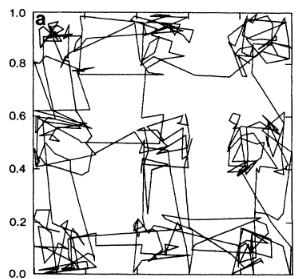
\includegraphics[width=150pt]{travelling_salesman.png}
    \caption{Modélisation du problème du voyageur de commerce}
\end{figure}

\section{Methode de Jacobi}

\subsection{Problème}

Soit $n \in \mathbb{N}$ , $A = (a_{i,j})_{i,j \in \llbracket 1,n \rrbracket^2}$ matrice carrée de taille $n$, $b = (b_i)_{i \in \llbracket 1,n \rrbracket}$ vecteur de taille $n$.

On cherche alors le vecteur $x = (x_i)_{i \in \llbracket 1,n \rrbracket}$ tel que :

\begin{equation} 
    \label{eq:probleme}
    Ax = b
\end{equation}

\subsection{Méthode de résolution}

Afin de résoudre ce problème, on va utiliser une méthode itérative appellée Méthode de Jacobi.\\

Tout d'abord, on va séparer la matrice $A$ en deux sous matrices $D$ et $R$ de la manière suivante :\\

\[
A = 
\begin{pmatrix}
    a_{1,1} & a_{1,2} & \cdots & a_{1,n} \\
    a_{2,1} & a_{2,2} & \cdots & a_{2,n} \\
    \vdots & \vdots & \ddots & \vdots \\
    a_{n,1} & a_{n,2} & \cdots & a_{n,n} 
\end{pmatrix}
=
\begin{pmatrix}
    a_{1,1} & 0 & \cdots & 0 \\
    0 & a_{2,2} & \cdots & 0 \\
    \vdots  & \vdots  & \ddots & \vdots  \\
    0 & 0 & \cdots & a_{n,n}
\end{pmatrix}
+
\begin{pmatrix}
    0 & a_{1,2} & \cdots & a_{1,n} \\
    a_{2,1} & 0 & \cdots & a_{2,n} \\
    \vdots  & \vdots  & \ddots & \vdots  \\
    a_{n,1} & a_{n,2} & \cdots & 0
\end{pmatrix}
\]\\

Notons $D$ la matrice diagonale, et $R$ la matrice du reste.
Comme la matrice $D$ est diagonale (qu'on suppose à coefficients nons nuls dans notre problème), $D$ est trivialement inversible d'inverse : \\

\[
D^{-1} =
  \begin{pmatrix}
  \frac{1}{a_{1,1}} & 0 & \cdots & 0 \\
  0 & \frac{1}{a_{2,2}} & \cdots & 0 \\
  \vdots  & \vdots  & \ddots & \vdots  \\
  0 & 0 & \cdots & \frac{1}{a_{n,n}}
 \end{pmatrix}
\]

On peut donc réécrire la formule \eqref{eq:probleme} de la manière qui suit :

\begin{align}
& (D + R)x = b\\
\Leftrightarrow \qquad & Dx = b - Rx \\
\Leftrightarrow \qquad & x = D^{-1}(b - Rx)
\end{align}

La Méthode de Jacobi est alors unt méthode itérative qui va chercher à trouver un point fixe à cet équation. On peut alors définir la suite $x^{(k)}, k \in \mathbb{N}$ telle que :

\[
    \left\{
    \begin{array}{l}
        x^{(0)} = \vec{0}\\
        x^{(k+1)} = D^{-1}( b - Rx^{(k)})
    \end{array}
    \right.
\]

L'avantage flagrant de cette méthode de calcul, est que les éléments n'ont aucune dépendance verticale. Elle est donc très simple à parallèliser. 

En effet,en écrivant la formule de récurrence pour un élement du vecteur $x^{(k+1)}$, on obtient :

\begin{align}
    \forall k \in \mathbb{N}, \forall i \in \llbracket 1,n \rrbracket, 
    \qquad x_{i}^{(k+1)} = \dfrac{1}{a_{i,i}}(b_i - \sum_{i \neq j}a_{i,j} x^{(k)}_j)
\end{align}

La seul contrainte devient alors que chaque processeur doit conna\^itre toutes les composantes de $x^{(k)}$ afin de pouvoir itérer, et il faut donc les communiquer, ce que nous feront en utilisant la bibliothèque MPI.

\subsection{Preuve et Convergence}

D'après le théorème de la méthode du point fixe, on sait que la suite $x_{n+1} = f(x_n)$ converge si la fonction $f$ est contractante ie $k$-lipshitzienne avec $k < 1$

Notons $C = -D^{-1}R$, $d = D^{-1}b$ et 
\begin{align*}
    \mathcal{F} : &\mathbb{R} \longrightarrow \mathbb{R} \\
    &u \longrightarrow Cu + d
\end{align*}

On veut trouver un condition nécessaire et suffisante pour que $\mathcal{F}$ soit une application contractante.\\
Or, on a :\\

Soit $a,b$ deux vecteurs dans $\mathbb{R}^n$,\\
\begin{align*}
    ||\mathcal{F}(a) - \mathcal{F}(b)|| &= ||Ca - Cb||\\
    &\leq||C||_{\infty} \cdot ||a-b||
\end{align*}

On doit donc avoir $||C||_{\infty} < 1$ ce qui revient à dire que le rayon spectral de la matrice $C$ noté $\rho(C)$ doit \^etre strictement inférieur à 1

On peut donc affirmer que :

\[
\lim_{k \to \infty}x^{(k)} = x \Leftrightarrow \rho(C) = \rho(-D^{-1}R) < 1
\]

Cherchons une condition simple suffisante pour affirmer que le rayon spectral de la matrice $C$ soit inférieur à 1.\\

Soit $\lambda$ valeur propre de $C$ ie $\forall y \in \mathbb{R}^n, Cy = \lambda y$

On a alors, $\forall (i,j) \in \llbracket 1,n \rrbracket^2$

\begin{align*}
    &||\lambda y||_{\infty} = |\sum_{j=1}^{n}c_{i,j}y_j\\
    \Leftrightarrow \qquad & \lambda||y||_{\infty} = |\sum_{j \neq i}\dfrac{a_{i,j}}{a_{i,i}}y_j|\\
    \Leftrightarrow \qquad & \lambda||y||_{\infty} = |\dfrac{1}{a_{i,i}}| \cdot |\sum_{j \neq i}a_{i,j}y_j|\\
    \Leftrightarrow \qquad & \lambda||y||_{\infty} \leq |\dfrac{1}{a_{i,i}}| \cdot \sum_{j \neq i}|a_{i,j}y_j|\\
    \Leftrightarrow \qquad & \lambda||y||_{\infty} \leq |\dfrac{1}{a_{i,i}}| \cdot \sum_{j \neq i}|a_{i,j}| \cdot ||y||_{\infty}\\
    \Leftrightarrow \qquad & \lambda \leq |\dfrac{1}{a_{i,i}}| \cdot \sum_{j \neq i}|a_{i,j}|
\end{align*}

Une condition suffisante pour que $\lambda < 1$ serait alors :

\[
\forall (i,j) \in \llbracket 1,n \rrbracket^2 \quad |a_{i,i}| > \sum_{i \neq j}|a_{i,j}|
\]
ie $A$ est à diagonale strictement dominante

\newpage 

\subsection{Vecteur erreur et résidu}

Afin de mesurer la convergence de la méthode de Jacobi (etd'avoir une condition d'arr\^et), on défini le vecteur erreur relative suivant :

\[
e^{(k+1)} = ||x^{(k+2)} - x^{(k+1)}||_{\infty} = ||C(x^{(k+1)} - x^{(k)})||_{\infty} = ||C||_{\infty}e^{(k)}
\]

On a donc $e^{(k)} = ||C||_{\infty}^ke^{(0)}$

On a de plus le vecteur erreur :

\[
\epsilon^{(k)} = ||x - x^{(k)}||_{\infty}
\]

$e^{(k)}$ est l'erreur relative de la méthode à l'itération $k$, mais comme on a pas connaissance du véritable vecteur $x$, on l'utilise comme référence pour le test d'arr\^et.

En effet, 

\begin{align*}
    e^{(k)} &= ||x^{(k+1)} - x^{(k)}||_{\infty}\\
    &= ||Cx^{(k)} + d - x^{(k)}||_{\infty}\\
    &= ||Cx^{(k)} + x - Cx - x^{(k)}||_{\infty}\\
    &= ||x - x^{(k)} - C(x - x^{(k)})||_{\infty}\\
    &= ||(-C + I)(x - x^{(k)})||_{\infty}
\end{align*}

On obtient alors par inégalité triangulaire: 

\[
e^{(k)} = ||I - C||_{\infty}\epsilon^{(k)} \leq \epsilon^{(k)} + ||C||_{\infty}\epsilon^{(k)}
\]

Et comme on a vu précedemment la norme infinie de la matrice $C$ est strictement inférieure à 1 on a donc :
\[
e^{(k)} \leq 2\epsilon^{(k)}
\]

On peut alors considérer que l'erreur relative est suffisament proche de l'erreur réelle pour l'utiliser comme test d'arr\^et.

\newpage

\section{Implémentation}

\subsection{Architecture}

Le projet est divisé en plusieurs sous-dossiers
\begin{itemize}
    \item \textbf{/lib} qui contient des librairies pour manipuler les matrices et les vecteurs ainsi que les opérations basiques de manipulation de ces deux structures de données.
    \item \textbf{/src} qui contient le fichier \textit{main} qui fait tourner le programme de l'agorithme de Jacobi.
    \item \textbf{/data} qui contient les fichiers des matrices et des vecteurs ainsi que les métadonnées contenant la taille des matrices considérées.
    \item \textbf{/bin} qui contientles binaires \textit{main} et \textit{test} afin de faire tourner le programme ou de tester les librairies
    \item \textbf{/test} qui contient le code source du binaire de test dont l'objectif est de tester les fonctions des lirbairies.
\end{itemize}
Le projet est de plus constitué d'un Makefile qui contient les procédures suivantes :
\begin{itemize}
    \item \textit{make all} (ou simplement \textit{make}) pour compiler les librairies, main et les tests 
    \item \textit{make test} pour compiler les tests 
    \item \textit{make clean} pour supprimer les fichiers objets
\end{itemize}

\subsection{Structures de données}

Dans ce projet, j'ai créé deux structures de données realitvement similaires pour les vecteurs et les matrices. Chaque structure dispose d'un type complexe qui lui est associé pour des raisons d'ergonomie.\\

Ces structures sont contenues dans les fichiers \texttt{lib/matrix.h} et \texttt{lib/vector.h}.\\

La structure Matrice est composé de deux entiers non signés pour les dimensions et d'un tableau de \textit{double} à 2 dimensions pour contenir les valeurs de la matrice.\\

\begin{lstlisting}
typedef struct Matrix{
    unsigned int col;
    unsigned int rows;
    double **matrix; 
}Matrix;
\end{lstlisting}

La structure Vecteur est très similaire mais n'a qu'une seule dimension:\\

\begin{lstlisting}
typedef struct Vector{
    unsigned int size;
    double **vector; 
}Vector;
\end{lstlisting}

\subsection{Librairies}

Ce projet est fourni avec 2 librairies situées dans les fichiers C du dossier \textbf{/lib}.

Les deux librairies ( Matrix et Vector ) sont analogues et possèdent des fonctions très similaires dont on remplacera le mot \textit{structure} par la structure qui correspond (matrix/vector):

\begin{itemize}
    \item \texttt{build\_structure} qui alloue dans la heap la structure avec la taille souhaitée
    \item \texttt{display\_structure} qui affiche le contenu algébrique de la structure
    \item \texttt{randomize\_structure} qui génère un contenu aléatoire (pas utilisée dans le projet en soit)
    \item \texttt{free\_structure} qui désalloue la structure de la heap et la reset
    \item \texttt{read\_structure\_from\_file} qui utilise un fichier pour remplir la structure\\
\end{itemize}

La fonction \texttt{read\_structure\_from\_file} est la seule fonction non triviale (plusieurs sous structures de fonctionnements internes). Elle peut échouer ($cf.$ partie \ref{err} page \pageref{err})

\begin{framed}
    \begin{algorithmic}
        \Function{read\_structure\_from\_file}{structure, filename, first\_line, size}
            \State Buffer of size 10000
            \State file $\gets$ open(filename)
            \If{file}
                \While{first\_line not reached}
                    \State buffer $\gets$ line
                \EndWhile
                \State build\_structure(structure, size)
                \If{build failed}
                    \State \Return error ENOMEM
                \EndIf
                \State structure $\gets$ file values
                \State \Return 0
            \Else
                \State \Return error ENOENT
            \EndIf
        \EndFunction
    \end{algorithmic}
\end{framed}

\subsection{Tests}

Le fichier de test ne verifie que le bon fonctionnement des librairies en générant des matrices et vecteurs de manière aléatoire et en utilisant un fichier de test.

\subsection{Données}

Pour le problème, trois fichiers de données différents sont nécessaires :
\begin{itemize}
    \item Un fichier de metadonnées (metadata.txt) qui contient les dimensions du problème
    \item Un fichier de matrice (matrix.txt) qui contient les données de la matrice $A$ séparées par des espaces
    \item Un fichier de vecteur (vector.txt) qui contient le vecteur $b$ du problème
\end{itemize}

\subsection{Compilation et Lancement}

Le Makefile n'est pas indispensable à la compilation du projet.
Les librairies doivent \^etre compilées puis liées au main (cela peut se faire en utilisant seulement gcc car les librairies n'utilisent pas MPI, mais mpicc est recommandé pour raison de compatibilité).\\

Le programme main est compilé en utilisant mpicc, le compilateur C de la librairie MPI. Les différents flags de compilations sont (viennent de gcc): 

\begin{itemize}
    \item \texttt{-Wall} qui active tout les messages de warning
    \item \texttt{-g} qui active les flags de debug
    \item \texttt{-O3} qui active toutes les optimisations de compilations
\end{itemize}

Pour lancer le programe : 

\texttt{mpirun -n n\_proc bin/main [-v] [-h?]}

\subsection{Programme principal}

Le programme principal est composé de \texttt{main.c} et \texttt{main.h}.

Celui ci à 3 fonctions :
\begin{itemize}
    \item \texttt{main} qui initialise le programme et résoud le système linéaire
    \item \texttt{product\_vector\_matrix} qui effectue le produit final en mode verbose pour verifier le résultat
    \item \texttt{usage} qui affiche l'usage de la Command Line Interface
\end{itemize}

Le programme peut recevoir les argument "-v" pour passer en mode verbose ou "-h/-?" pour afficher l'usage.

Les fichiers de données sont hardcodés dans le code source, mais cette partie est facilement modifiable pour pouvoir spécifier le chemin des fichiers en question.\\

Ce programme effectue la méthode de Jacobi en asynchrone utilisant :

\begin{itemize}
    \item MPI\_Isend qui envoi des données de manière asynchrone 
    \item MPI\_Irecv qui reçoit des données de manière asynchrone
    \item MPI\_Wait qui permet d'attendre  la réalisation d'un requ\^ete asynchrone (send ou recv)\\
\end{itemize}

Le principe de communication est le suivant :\\

Les processeurs disposent d'une variable \texttt{mtx} qui contient une sous-matrice et \texttt{vect} le sous-vecteur de $b$ associée à la sous matrice suivant un découpage par lignes distribué de manière équilibré sur ceux-ci.

Par exemple, une matrice $3 \times 3$ sur $2$ processeurs serait découpées avec la distribution de lignes suivantes :

\begin{align*}
    &\begin{pmatrix}
        a_{1,1} & a_{1,2} & a_{1,3}\\
        a_{2,1} & a_{2,2} & a_{2,3}\\
    \end{pmatrix} \\
    &\begin{pmatrix}
        a_{3,1} & a_{3,2} & a_{3,3}\\
    \end{pmatrix}
\end{align*}


Ensuite, chaque processeur dispose d'une variable \texttt{global\_result} qui contient $x^{(k)}$ à l'étape $k$ et de \texttt{local\_result} qui après itération contiendra les sous vecteurs de $x^{(k+1)}$ à l'étape $k$.\\

Il y'a également un tableau \texttt{continue\_iterate} qui pour chaque ligne de chaque processeur contient un booleén qui permet de décider si l'on continue d'itérer sur la ligne en question.

Au début de chaque itération, les processeurs envoient la valeur locale de \texttt{global\_result} dans lequel on a stocké l'itération que l'on viens de terminer, et l'on complète cette variable en recevant la valeur locale des autres processeurs.\\

Les appels à la fonction MPI\_Irecv sont suivi généralement d'un appel à MPI\_Wait qui va attendre que la reception soit effective car elle est nécéssaire à l'opération qui suit.\\

En revanche nous ne mettons pas de MPI\_Wait après MPI\_Isend car les données ne sont mutés qu'après récéption de la données suivante, et la requ\^ete d'envoi sera donc terminée à ce moment.\\

Ensuite on applique la formule de récurrence sur ces nouvelles données que l'on stock dans \texttt{local\_result}.\\

Pour le test d'arr\^et, comme nous somme en norme infinie, on peut calculer l'erreur relative de chaque composante $e^{(k)}_{i} = x^{(k+1)}[i] - x^{(k)}[i]$

On va alors tester chaque ligne de chaque processeur et ne continuer l'itération de celles-ci que si la convergence est atteinte :

\[
e^{(k)}_{i} \leq 1.10^{-6}
\]

Pour cela, on modifie à l'interieur de chaque processeur la tableau de booléens \texttt{continue\_iterate}, puis une fois que le tableau ne contiens que des \texttt{false}, on envoi la valeur false au processeur root pour que celui ci fasse un masque binaire de tout les autres pour décider de stoper la boucle principale. La limite d'itérations fixée à 500 est arbitraire et pourrait certainement \^etre abaissée.

\subsection{Erreurs} \label{err}

L'architecture de code de ce programme suit les standard de développement basés sur le status d'une opération. En effet, dans ce programme beaucoup de fonctions sont succeptibles d'échouer (la manipulation de fichier, l'allocation mémoire, ...).\\

Dans cette optique, les fonctions des librairies  utilisent des pointeurs sur les variables, qui sont alors mutées en place, et les fonctions renvoient un code stipulant la réussite ou l'échec de l'opération an utilisant les code d'erreurs standards de la librairie \texttt{errno.h}.\\

Les codes utilisés ici sont :
\begin{itemize}
    \item Code Erreur 2, \texttt{ENOENT} : "No such file or directory"
    \item Code Erreur 12, \texttt{ENOMEM} : "Out of memory"
    \item Code Erreur 22, \texttt{EINVAL} : "Invalid argument"
    \item Code Erreur -1 : Erreur générique
\end{itemize}

\newpage

\section{Résultats}

\subsection{Mesures des performances}

Pour mesurer les performances génerales du programme, j'ai fait tourner le script bash suivant

\begin{lstlisting}[language=bash]
    for proco in {1..8}                                      
    do                
        time mpirun -n $proco bin/main | grep "total"
    done
\end{lstlisting}

J'ai mesuré les performances du programme sur différents sets de données (donc ceux fournis avec le projet)
\begin{itemize}
    \item Les données fournies (de taille 7)
    \item une matrice creuse de taille 20
    \item une matrice creuse de taille 200
    \item une matrice creuse de taille 1000\\
\end{itemize}

Les matrices utilisées n'ont pas étés fournies mais peuvent \^etre générées à l'aide du script python fourni

Les résultats sont présentés dans l'image suivante :

\begin{figure}[h]
    \centering
    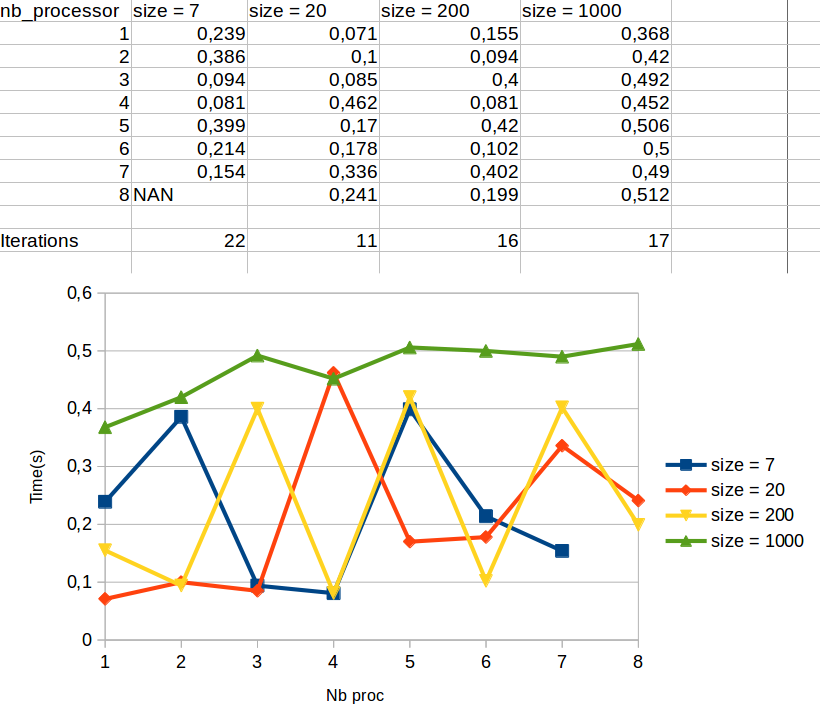
\includegraphics[width=250pt]{perf.png}
    \caption{Performances et vitesse de convergence du programme avec différents sets de données}
\end{figure}

\subsection{Génération de matrices creuses de grande taille}

Afin de générer des matrices de grandes tailles pour tester les performances du programme, j'ai écrit un script python qui construisait des matrices creuses aléatoires afin de conserver la caractéristique de matrice à diagonale strictement dominante.\\

Ce programme ce situe dans le dossier \textbf{/data} et se nomme \texttt{generate\_random\_mtx\_vec.py}.\\

Lancement : \texttt{python3 generate\_random\_mtx\_vec.py <size>}\\

Il génère une matrice carré et un vecteur de taille \textbf{argv[1]}, avec des coefficients entre 100 et 150 pour la diagonale, et entre -2 et 2 pour les 9 lignes de chaque coté de la diagonale ( on a bien $2*2*9 < 100 $)

\subsection{Analyse des performances et des résultats}

Les résultats d'analyse des performances sont à première vu perturbants. En effet, on remarque que pour la méthode de Jacobi purement asynchrone, la performance n'augmente  pas liénairement en fonction du nombre de processeur.\\

Cela peut s'expliquer par l'overhead d\^u à la communication entre les processeurs que j'ai obligé à attendre avant de muter les données; plus on augmente le nombre de processeurs plus le nombre de communications et donc d'attentes est important.\\

On observe par contre de manière quasi-systématique unemeilleur performance sur un nombre de processeur pair par rapport à sur un nombre de processeurs impair.\\

Une réinjection de la solution trouvée pour le set de données fourni dans l'équation d'origine en utilisant la fonction de produit vectoriel activé en mode debug, nous obtenons un résultat encourageant :

\begin{figure}[h]
    \centering
    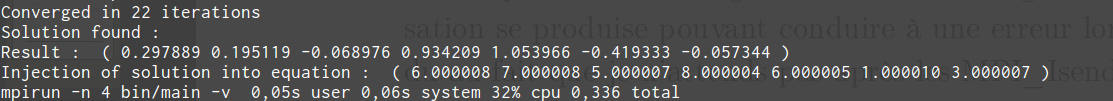
\includegraphics[width=350pt]{convergence.png}
    \caption{Réinjection de la solution itérative dans l'équation}
\end{figure}

Le vecteur d'origine étant $b = (6,7,5,8,6,1,3)$\\

Je n'ai pas testé le debug sur des matrices de grande taille, mais il est probable qu'une désynchronisation se produise pouvant conduire à une erreur lors du calcul de l'erreur relative (éventuellement du au fait que je n'attends pas après les MPI\_Isend).

\newpage

\section{Conclusion}

J'ai réalisé un programme en $C$ utilisant le librairie MPI afin d'utiliser la Méthode de Jacobi parallélisée de manière asynchrone pour résoudre un système linéaire.\\

Ce programme a fourni des résultats très satisfaisants, convergeant rapidement et semblant réster relativement synchronisé.\\

J'ai beaucoup appris, surtout sur la manière de paralléliser un programme en langage bas niveau, et j'ai pu me réaffirmer sur ma ma\^itrise du langage (m\^eme si cela ne fait peut-\^etre pas partie des objectifs du cours).\\

J'ai de plus plusieurs remarques sur les pistes d'améliorations du programme ou de la démarche :\\

Je n'ai réalisé que l'implémentation purement asynchrone du programme, j'aurais pu le rendre plus modulaire et lui permettre de fonctionner en synchrone ou en asynchrone + MPI\_Barrier afin de comparer les différence performance et de m'assurer de l'absence de désynchronisations.\\

Je n'ai pas permis la modification desfichier de données via command line arguments, cela aurait rajouté de l'implémentation inutile de vérification d'existence de fichier, etc ..., Ce qui n'est pasl'objectif de l'exercice.\\
De plus, le script python génère des fichiers nommés \texttt{object\_t.txt} (object pouvant \^etre matrix, vector ou metadata), alors que dans le code source, nous chargeons \texttt{object.txt}.\\
Cela peut \^etre aisément changé dans le code source, ou alors il faut remplacer les fichier de données fournis.\\

Enfin, j'ai remarqué que le temps d'execution variait d'une fois à l'autre, ce que je n'ai pas réussi à expliquer.

\end{document}